\documentclass[12pt]{article}

\usepackage[margin=1in]{geometry}
\usepackage{tikz}
\usetikzlibrary{shapes.geometric, arrows.meta, positioning, calc}
\usepackage{parskip}
\usepackage{fancyhdr}
\usepackage{hyperref}
\usepackage{longtable}
\usepackage{booktabs}
\usepackage{amssymb}
\usepackage{graphicx}

\hypersetup{colorlinks=true, linkcolor=blue, urlcolor=blue}

\pagestyle{fancy}
\fancyhf{}
\rhead{Campus Resource Booking \& Check-In System}
\lhead{Workflow Diagram}
\rfoot{Page \thepage}

\tikzset{
  actor/.style={
    rectangle, rounded corners=6pt,
    minimum width=2.7cm, minimum height=0.85cm,
    text centered, align=center, draw=black!70, fill=blue!10,
    font=\small\bfseries
  },
  service/.style={
    rectangle, rounded corners=4pt,
    minimum width=3.5cm, minimum height=0.9cm,
    text centered, align=center, draw=black!70, fill=orange!20,
    font=\small
  },
  middleware/.style={
    rectangle, rounded corners=4pt,
    minimum width=3.5cm, minimum height=0.9cm,
    text centered, align=center, draw=black!70, fill=yellow!30,
    font=\small
  },
  db/.style={
    cylinder, shape border rotate=90,
    aspect=0.28,
    minimum width=3.0cm, minimum height=1.3cm,
    text centered, align=center, draw=black!70, fill=green!15,
    font=\small\bfseries
  },
  arrow/.style={-{Stealth[length=6pt]}, thick, draw=black!70},
  dasharrow/.style={-{Stealth[length=6pt]}, thick, dashed, draw=black!50},
}

\title{
    \vspace{2cm}
    {\Large Workflow Diagram} \\[1em]
    {\LARGE \textbf{Campus Resource Booking \& Check-In System}} \\[2em]
    {\large CS3338 --- Group 1} \\[0.5em]
    {\normalsize Version 4.0}
    \vspace{2cm}
}
\author{DevOps / QA}
\date{May 15, 2025}

\begin{document}

\maketitle
\thispagestyle{empty}
\newpage

% -------------------------------------------------------
\section*{Versions Table}

\begin{longtable}{|p{1.4cm}|p{2.4cm}|p{3.5cm}|p{6.5cm}|}
\hline
\textbf{Ver.} & \textbf{Date} & \textbf{Author(s)} & \textbf{Changes} \\
\hline
1.0 & Feb 2, 2025  & DevOps/QA & Initial workflow diagram --- basic 3-tier architecture. \\
\hline
2.0 & Mar 2, 2025  & DevOps/QA & Added JWT auth flow, RBAC middleware layer, booking conflict path. \\
\hline
3.0 & Apr 6, 2025  & DevOps/QA & Added check-in flow, no-show background job, admin analytics path. \\
\hline
4.0 & May 15, 2025 & DevOps/QA & Final revision. Added rate limiter, full access control table, data flow description updated. \\
\hline
\end{longtable}
\newpage

% -------------------------------------------------------
\section*{System Architecture Overview}

\begin{center}
\resizebox{0.92\textwidth}{!}{%
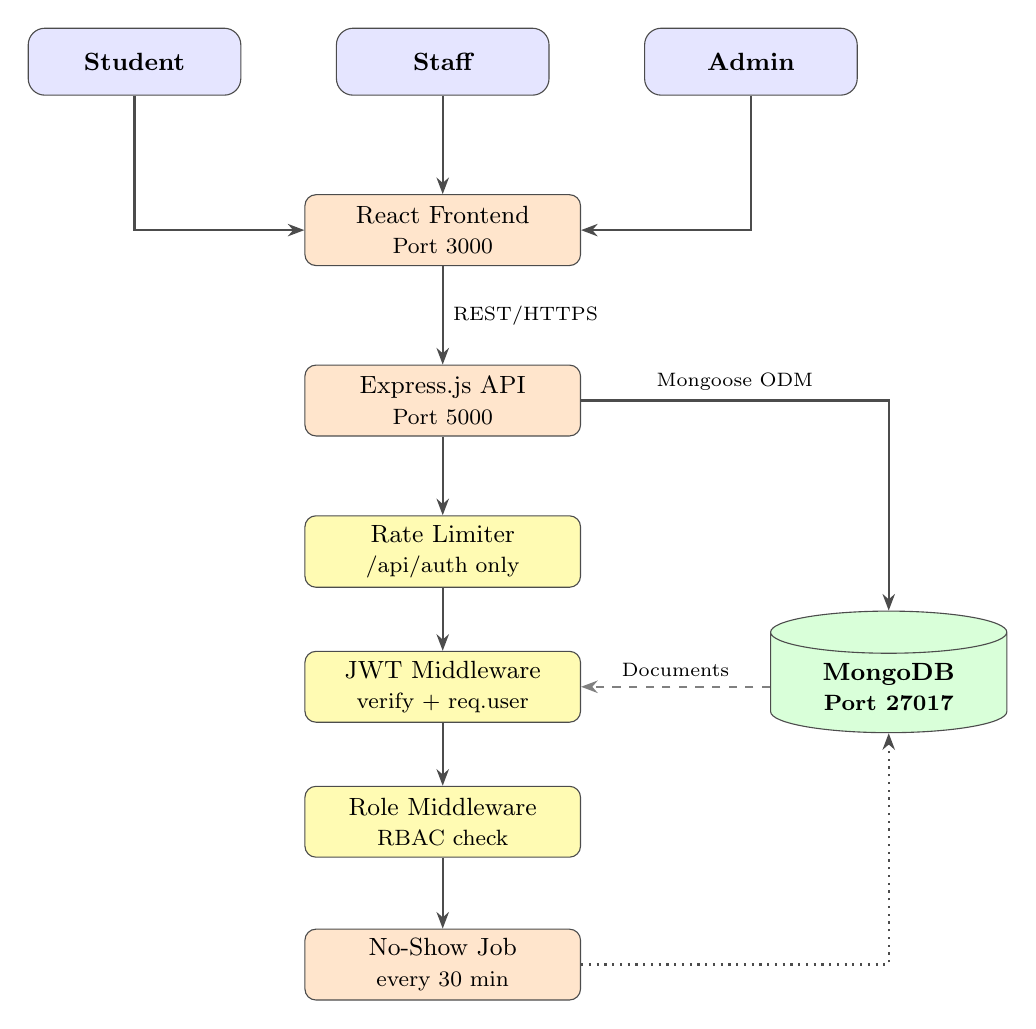
\begin{tikzpicture}[node distance=1.25cm and 1.6cm]

% --- User roles ---
\node[actor] (student) {Student};
\node[actor, right=1.2cm of student] (staff) {Staff};
\node[actor, right=1.2cm of staff] (admin) {Admin};

% --- Frontend and backend ---
\node[service, below=1.25cm of staff] (frontend)
  {React Frontend\\{\footnotesize Port 3000}};

\node[service, below=1.25cm of frontend] (backend)
  {Express.js API\\{\footnotesize Port 5000}};

% --- Middleware stack ---
\node[middleware, below=1.0cm of backend] (ratelimit)
  {Rate Limiter\\{\footnotesize /api/auth only}};

\node[middleware, below=0.8cm of ratelimit] (authmw)
  {JWT Middleware\\{\footnotesize verify + req.user}};

\node[middleware, below=0.8cm of authmw] (rolemw)
  {Role Middleware\\{\footnotesize RBAC check}};

% --- Database and background job ---
\node[db, right=2.4cm of authmw] (mongo)
  {MongoDB\\{\footnotesize Port 27017}};

\node[service, below=0.9cm of rolemw] (noshowjob)
  {No-Show Job\\{\footnotesize every 30 min}};

% --- User arrows ---
\draw[arrow] (student.south) |- (frontend.west);
\draw[arrow] (staff.south) -- (frontend.north);
\draw[arrow] (admin.south) |- (frontend.east);

% --- Main request path ---
\draw[arrow] (frontend.south) -- node[right, font=\scriptsize]{REST/HTTPS} (backend.north);
\draw[arrow] (backend.south) -- (ratelimit.north);
\draw[arrow] (ratelimit.south) -- (authmw.north);
\draw[arrow] (authmw.south) -- (rolemw.north);

% --- Database path ---
\draw[arrow] (backend.east) -| node[pos=0.25, above, font=\scriptsize]{Mongoose ODM} (mongo.north);
\draw[dasharrow] (mongo.west) -- node[above, font=\scriptsize]{Documents} (authmw.east);

% --- Background job path ---
\draw[arrow] (rolemw.south) -- (noshowjob.north);
\draw[arrow, dotted] (noshowjob.east) -| (mongo.south);

\end{tikzpicture}%
}
\end{center}

\vspace{1em}
\textit{Dotted arrow = background process not triggered by a user request.}

% -------------------------------------------------------
\section*{Step-by-Step Data Flow}

\begin{enumerate}
    \item \textbf{Browser request} --- User opens \texttt{http://localhost:3000}. Docker serves the React static bundle from the frontend container.

    \item \textbf{Authentication} --- User submits login form. React sends \texttt{POST /api/auth/login} to the Express backend. The Rate Limiter middleware checks request frequency, with a maximum of 10 requests per IP address every 15 minutes. On pass, the controller verifies the bcrypt password hash and returns a signed JWT.

    \item \textbf{Token storage} --- React stores the JWT in \texttt{localStorage} and registers an Axios interceptor that appends \texttt{Authorization: Bearer token} to every outgoing request.

    \item \textbf{Protected request} --- User performs an action such as booking a room. React sends \texttt{POST /api/bookings}. The JWT Middleware verifies the token signature and expiry; it attaches the user ID and role to \texttt{req.user}.

    \item \textbf{Role enforcement} --- The Role Middleware checks that \texttt{req.user.role} is in the set of permitted roles for the route. Unauthorized roles receive HTTP 403.

    \item \textbf{Business logic} --- The booking controller calls \texttt{conflictCheck.js}, which queries MongoDB for any overlapping confirmed bookings for the same resource. If no conflict exists, a Booking document is written to MongoDB.

    \item \textbf{Check-in flow} --- Student clicks Check In. \texttt{PUT /api/bookings/:id/checkin} validates that the current server time is within the check-in window before updating the booking status to \texttt{checked-in}.

    \item \textbf{No-show detection} --- A \texttt{setInterval} function in \texttt{server.js} runs every 30 minutes and bulk-updates any confirmed bookings whose check-in windows have passed without a check-in to status \texttt{no-show}.

    \item \textbf{Analytics} --- Admin requests \texttt{GET /api/admin/analytics}. The controller runs MongoDB aggregation pipelines to compute booking counts, check-in rates, and daily time-series data. Results are returned as JSON to the React admin dashboard for rendering with recharts.

    \item \textbf{Response cycle} --- All responses return JSON with appropriate HTTP status codes. React updates component state and re-renders the UI without a full page reload.
\end{enumerate}

% -------------------------------------------------------
\section*{Access Control Summary}

\begin{center}
\begin{tabular}{|l|c|c|c|}
\hline
\textbf{Action / Endpoint} & \textbf{Student} & \textbf{Staff} & \textbf{Admin} \\
\hline
Register / Login & \checkmark & \checkmark & \checkmark \\
Browse resources & \checkmark & \checkmark & \checkmark \\
Create booking & \checkmark & \checkmark & \checkmark \\
Cancel own booking & \checkmark & \checkmark & \checkmark \\
Check in within window & \checkmark & \checkmark & \checkmark \\
Create / edit resources & --- & \checkmark & \checkmark \\
View bookings for own resources & --- & \checkmark & \checkmark \\
View all bookings platform-wide & --- & --- & \checkmark \\
Cancel any booking & --- & --- & \checkmark \\
Manage all users & --- & --- & \checkmark \\
View analytics dashboard & --- & --- & \checkmark \\
\hline
\end{tabular}
\end{center}

% -------------------------------------------------------
\section*{Docker Network Topology}

All containers run on the \texttt{crbs\_network} bridge network created by \texttt{docker-compose}. Service names such as \texttt{mongo}, \texttt{backend}, and \texttt{frontend} are used as DNS hostnames within the network.

\begin{center}
\begin{tabular}{|l|l|l|l|}
\hline
\textbf{Container} & \textbf{Image} & \textbf{Internal Port} & \textbf{Host Port} \\
\hline
crbs\_frontend & node:18-alpine & 3000 & 3000 \\
crbs\_backend & node:18-alpine & 5000 & 5000 \\
crbs\_mongo & mongo:6 & 27017 & 27017 \\
\hline
\end{tabular}
\end{center}

\end{document}